\chapter{Técnicas de luz estruturada e \emph{Time Of Flight}}\label{cap:kinect}
%======================================================================================

\section*{Introdução}

A técnica de luz estruturada é um
\textbf{método fotogramétrico ativo} que consegue determinar a localização de objetos
no alcance do sensor de infra-vermelho, a partir de alterações nos padrões conhecidos de um projetor 
infra-vermelho. Um exemplo recente de escaneador de luz estruturada de baixo custo
é o Kinect versão~\cite{smisek20133d}, que também serve como base para uma
série de scanners que utilizam o mesmo hardware. Uma vantagem clara em relação
aos escaneadores a \emph{laser} é a velocidade e o baixo custo; uma desvantagem
é a precisão, conforme discutido mais adiante.  Existe também, um outro método
fotogramétrico ativo denominado\emph{Time of Flight}~\cite{gokturk2004time},
que em vez de padrões infra-vermelho ou laser, emite fótons a cada pixels, que
viajam na velocidade da luz. O valor resultante da diferença da
emissão e do retorno dos fótons aos
detectores é utilizado na criação de uma distribuição de probabilidade 
localizando o evento detectado a uma distância do eixo do escaneador.

Até recentemente, a técnica ToF foi extremamente cara e restrita a baixas resoluções, devido à
necessidade de equipamento capaz de medir fotons refletidos em uma escala de
picosegundos. Tal técnica foi barateada em ordens de magnitude pela indústria
de entretenimento, no lançamento recente do Kinect versão
2~\cite{lachat2015first,valgma20163d}. Além do baixo custo permitido pelo
Kinect 2, uma vantagem desta técnica é a alta velocidade de escaneamento e
maior robustez dos resultados se comparado à técnica de luz estruturada e mesmo escaneadores a \emph{laser}.
No enanto, ela não pode ser aplicada com confiabilidade em ambientes abertos,
e não supera a precisão de um bom escaneador a \emph{laser}. Note-se que, no entanto, escaneadores a \emph{laser} Não são adequados para aplicações em tempo real; porém, para o nosso objetivo de preservação de patrimônio,
o requisito de escaneamento em tempo real é secundário, sendo desejável apenas para aplicações em que uma previsão rápida da reconstrução 3D é desejada pelo arqueólogo, ou para realidade aumentada.
A seguir, discutimos essas tecnologias de reconstrução 3D ativas em maiores detalhes.

\section{Kinect}

\subsection*{Introdução}

Criado pela Microsoft para fins recreativos (como no console de videogame XBox, por
exemplo), o Kinect se tornou uma das mais conhecidas ferramentas de reconstrução 3D no
cenário atual. Sua primeira versão (Kinect V1)~\ref{fig:kinectv1}, ainda atual, utiliza uma
técnica similar à empregada no projeto \emph{Digital Michelangelo} da Universidade de Stanford, com luz
estruturada, porém, diferentemente dos escaners a \emph{laser}, o Kinect é mais rápido e tem um
custo monetário baixo, acessível ao público em geral (desde entusiastas
e amadores até profissionais da área). 

O Kinect versão 2 é composto de uma câmera RGB-D (\emph{red, green, blue} e
\emph{depth}) e utiliza uma projeção de fótons, sendo mais robusto que seu
antecessor, para ambientes fechados e para fins de escaneamento de formas
humanas (como esqueleto, músculos, e até mesmo para medir o batimento cardíaco, por exemplo). Devido à
técnica empregada para reconhecimento 3D \emph{Time of Flight},
ele é muito sensível às texturas presentes no objeto, ou seja, esculturas
com diferentes superfícies, diferentes refletâncias, lambertianas ou
especulares, por exemplo, podem acarretar em problemas ou buracos nas reconstruções. Além
disso, existem outros obstáculos, como a dificuldade em que o fóton emitido 
rebate em várias superfícies antes de ser detectado pelo sensor. 
Portanto, para o uso em áreas externas, a primeira versão do Kinect se sai melhor.

O Kinect versão 1 é composto por duas câmeras: uma RGB apenas para cores e aparência,
e outra câmera infra-vermelho para profundidade, atuando em sincronia com um projetor de padrões em infra-vermelho (IR ou \emph{infra-red}). O projetor IR lança uma matriz de padrões que já é previamente
conhecida pelo sistema do Kinect, e, a partir disso, qualquer deformação deste
padrão é captada pela câmera IR, o que identifica se um objeto está no alcance
dos sensores ou não. O espectro infra-vermelho é utilizado por não ser percebido pela visão humana.
A resposta é composta por 3 saídas: uma imagem de intensidades IR, uma RGB e a profundidade de cada pixel. 

A seguir, será usado o termo ``Kinect'' para o Kinect versão 1, pois este é ainda
o modelo mais utilizado na literatura para o escaneamento de objetos, conforme
é o foco deste trabalho, em vez do rastreamento em tempo real para entretenimento, que é
dominado pelo Kinect versão 2.

\begin{figure}[!h]
	\centering
	%   \includegraphics[width=1.0\linewidth]{figs/3d-curve-sketch/system-diagram.eps}
	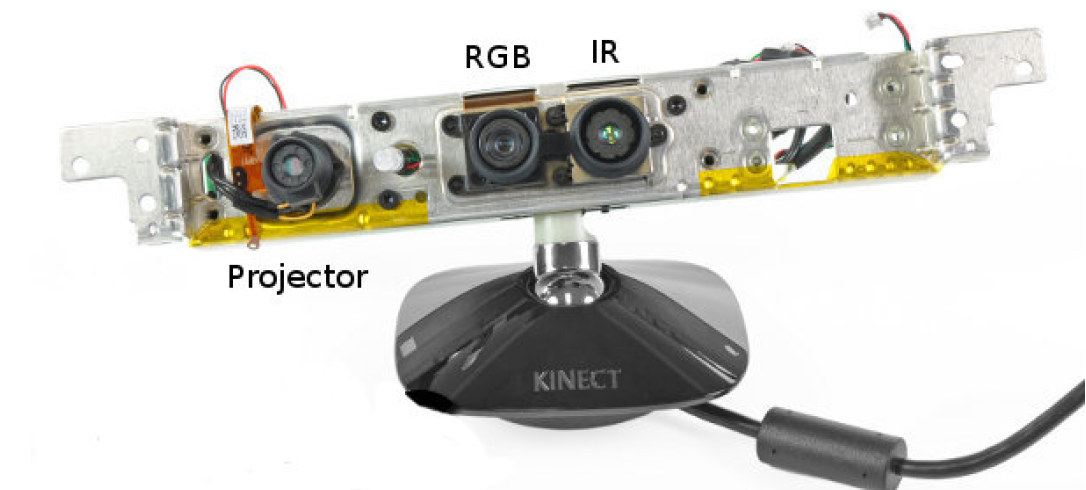
\includegraphics[width=0.5\linewidth]{figs/kinect.png}
	\caption{%
  Imagem de um Kinect V1 aberto, constituído de uma câmera infra-vermelho (IR -
  \emph{Infra-Red}), uma câmera RGB e um projetor IR.
  \protect\cite{smisek20133d}.
	}\label{fig:kinectv1}
\end{figure}

\subsection*{Processo de calibração}

A principal saída do Kinect é correspondente à profundidade da
cena. Na realidade, em vez de providenciar uma profundidade $Z$, ele retorna uma profundidade
inversa, $D$. Essa informação é construída a partir da triangulação
da imagem IR com o padrão conhecido do projetor.

\begin{figure}[!h]
	\centering
	%   \includegraphics[width=1.0\linewidth]{figs/3d-curve-sketch/system-diagram.eps}
	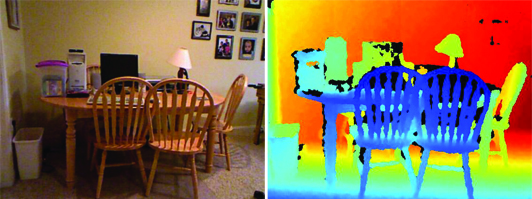
\includegraphics[width=1\linewidth]{figs/profundidadekinect.png}
	\caption{%
  Exemplo de como é a saída de uma imagem interpretada pelo Kinect, onde cada
  disposta na imagem corresponde à profundidade ou distância da cena para
  o Kinect, e preto corresponde a pontos sem informação confiável.
	\cite{Silberman:ECCV12}.
	}\label{fig:profKinect}
\end{figure}
 
Na literatura, foram realizados alguns experimentos associando o uso do Kinect V1 como um
escaneador de baixo custo em reconstruções~\cite{smisek20133d}, tarefa para a qual não foi
originalmente projetado. Primeiramente, foi executada uma calibração do
Kinect para este tipo de reconstrução, onde, a partir de experimentos, o sistema
foi modelado como
\begin{equation}
\label{eq:kinectCalibracao}
q(z)=2.73z^{2}+0.74z-0.58,
\end{equation}
onde $z$ é a profundidade em metros, e $q$ a quantização, em milímetros.
O modelo geométrico do Kinect foi criado com um sistema multi-ocular
(\emph{multi-view}) considerando o RGB, IR e a profundidade.
\begin{gather} 
\label{eq:matrix}
\begin{bmatrix}
u\\
v\\
1
\end{bmatrix} 
= k
\begin{bmatrix}
s\\
t\\
1
\end{bmatrix}
\end{gather}

\begin{gather} 
\begin{bmatrix}
s\\
t\\
1
\end{bmatrix} 
= 
\underbrace{(1 + k_1r^2 + k_2r^4 + k_5r^6) 
\begin{bmatrix}
p\\
q\\
0
\end{bmatrix} }_{\text{distorção radial}} 
+
\underbrace{
\begin{bmatrix}
2k_3pq+k_4(r^2+2p^2)\\
2k_4pq+k_3(r^2+2q^2)\\
1
\end{bmatrix} }_{\text{distorção tangencial}}
\label{eq:distorcaoKinect}
\end{gather}

\begin{gather}
r^2 = p^2+q^2, 
\begin{bmatrix}
pz\\ 
qz\\ 
z
\end{bmatrix} = R(X-C),
\label{eq:relacaoKinect}
\end{gather}
onde $k_n$ é o parâmetro de distorção, matriz de calibração da câmera $K$,
rotação $R$ e centro de projeção $C$.
A profundidade é associada à geometria da câmera IR. que retorna a profundidade inversa ao longo do eixo $z$.
Os valores de $u$ e de $v$ são dados pela equação~\ref{eq:distorcaoKinect}, %(substitui-se o vetor [s, t, 1] em 2), X é o ponto coordenada 3D, c1 e c0 parâmetros do modelo.

\begin{gather} 
X_{IR} = \frac{1}{c_1 d + c_0}dis^{-1}\left ( K^{-1}_{IR}
\begin{bmatrix}
x+u_0\\ 
y+v_0\\ 
1
\end{bmatrix},k_{IR} 
\right )
\label{eq:distKinect}
\end{gather}

\begin{equation}
\label{eq:finalKinect}
u_{RGB} = K_{RGB} dis(R_{RGB}(X_{IR} - C_{RGB}),k_{RGB}).
\end{equation}

Associamos o sistema de coordenadas do Kinect com a câmera IR e,
consequentemente, $R_{IR} = I$ (identidade) e $C_{IR} = 0$.  O ponto 3D $X_{IR}$
é construído a partir da medição de $[x,y,d]^\top$ da equação~\ref{eq:distKinect} e
produz uma imagem RGB, Equação~\ref{eq:finalKinect}.

Em \ref{eq:distKinect}, $dis$ é a distorção, proveniente de
\ref{eq:distorcaoKinect}, $k_{IR}$ e $k_{RGB}$ são, respectivamente, distorção
relacionada à IR e à RGB.  $K_{IR}$ é a matriz de calibração da câmera IR,
$K_{RGB}$ é a matriz de calibração da câmera RGB. $R_{RGB}$ e $C_{RGB}$ são, a
matriz de rotação e de centro da câmera RGB, respectivamente.

A calibração ocorreu usando o mesmo alvo nas câmeras IR e RGB, mesmos pontos 3D,
e consequentemente, a mesma posição relativa das câmeras.  O sistema de
coordenadas global do Kinect faz a posição relativa da câmera igual a $R_{RGB}$,
$C_{RGB}$.

Também foi observado que existe um deslocamento entre imagem IR e a imagem da
profundidade criada pelo Kinect. Para contornar este problema, uma série de
experimentos foram executados, gerando \ref{tab:deslocamentoKinect}.

\begin{table}[!h]
\centering
\caption{Valores de deslocamentos e sua média}
\label{tab:deslocamentoKinect}
\begin{tabular}{|l|l|l|l|l|l|}
\hline
Imagem & 1   & 2   & 3   & 4   & Média \\ \hline
$u_0$  & 2,8 & 2,9 & 3,0 & 3,4 & 3,0   \\ \hline
$v_0$  & 3,0 & 2,7 & 2,8 & 3,1 & 2,9   \\ \hline
\end{tabular}
\end{table}

\begin{figure}[!h]
	\centering
	\subfloat[Sem o alinhamento]{\label{fig:deslocamentokinectA}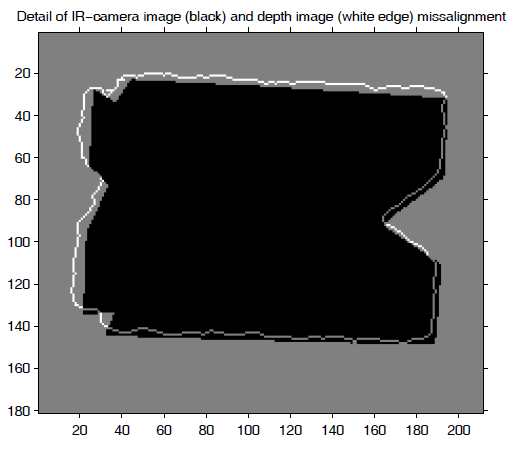
\includegraphics[width=0.3\linewidth]{figs/deslocamentokinectA.png}}
	\subfloat[Com o alinhamento]{\label{fig:deslocamentokinectB}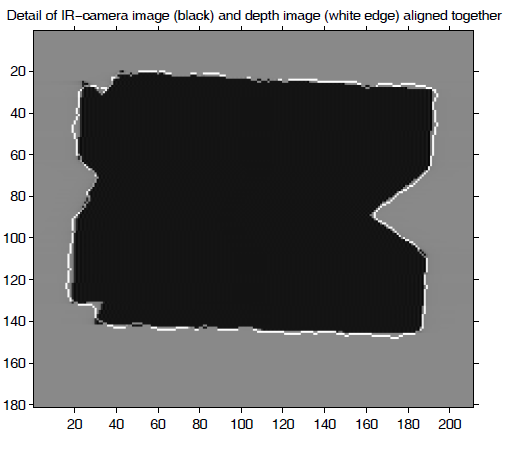
\includegraphics[width=0.3\linewidth]{figs/deslocamentokinectB.png}}
	\caption{%
	Representação visual do acerto do deslocamento. A parte em preto é a imagem IR e o contorno em branco é a imagem de profundidade do alvo.
	\protect\cite{smisek20133d}
	}\label{fig:deslocKinect}
\end{figure}

Foi observado que após a calibração, o Kinect gerava erros residuais complexos, que para compensar esse erro residual, foi criada uma correção em $z$, onde é subtraído da coordenada $Z_{IR}$ de \ref{eq:distKinect}.
Para validar essa correção, a correção-z das imagens foram construídas a partir dos resíduos das imagens ímpares e aplicadas nas pares, e o vice-versa. Depois da aplicação da correção-z , a media dos erros diminuiu aproximadamente 0,25mm.
Como parâmetro de comparação, foram dispostas 2 câmeras diferentes, no mesmo ambiente do Kinect.

\begin{figure}[!h]
	\centering
	%   \includegraphics[width=1.0\linewidth]{figs/3d-curve-sketch/system-diagram.eps}
	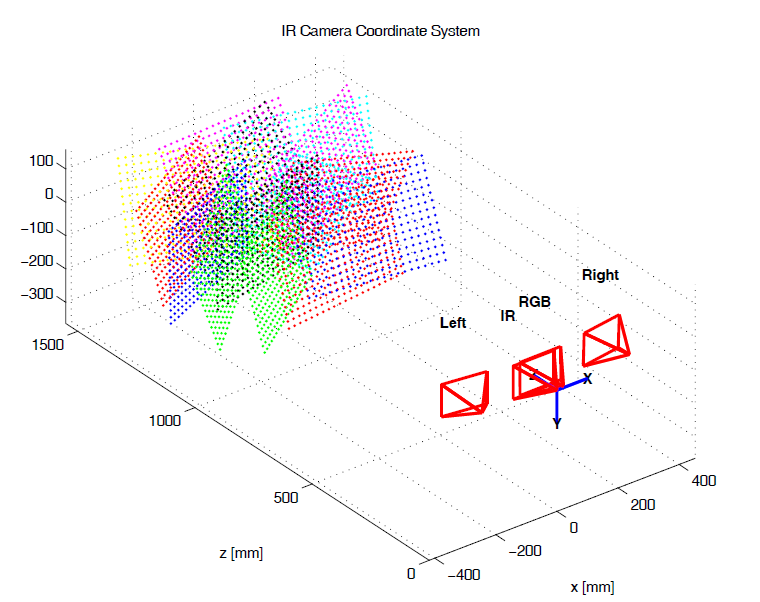
\includegraphics[width=0.5\linewidth]{figs/ambientekinect.png}
	\caption{%
	Posição e orientação do Kinect (com as câmeras IR e RGB) e o par estéreo SLR (\emph{Left}, \emph{Right}) em conjunto com pontos de calibração 3D reconstruídos em alvos de calibração planar.
	\protect\cite{smisek20133d}.
	}\label{fig:ambienteKinect}
\end{figure}

\begin{table}[htbp]
\caption{Resultados dos testes executados no ambiente descrito anteriormente}
\label{tab:resultadosKinect}
\begin{center}
\begin{tabular}{|c|c|c|c|}
\hline
\multirow{2}{1.5cm}{Método}& \multicolumn{3}{p{5cm}|}{Erro geométrico $e$ [mm]} \bigstrut \\
\cline{2-4} & \multicolumn{1}{c|}{$\mu$($e$)} & \multicolumn{1}{c|}{$\sigma$($e$)} & \multicolumn{1}{c|}{max($e$)} \bigstrut \\ \hline
SLR Stereo & 1,57 & 1,15 & 7,38 \bigstrut \\ \hline
Kinect & 2,39 & 1,67 & 8,64 \bigstrut \\ \hline
SR-4000 & 27,62 & 18,20 & 133,85 \bigstrut \\ 
\hline
\end{tabular}
\end{center}
\end{table}

\subsection*{Uso do Kinect com \emph{Structure from Motion}}

Com o sistema calibrado, o Kinect foi testado usando técnicas \emph{Structure from Motion}, onde a figura a seguir compara a superfície 3D de nuvem de pontos com uma com Kinect. 

O resultado é tão bom quanto ao mais acurado \emph{Multi-View Stereo}.

O Kinect tem a capacidade e, com o procedimento de calibração, é possível combiná-lo com técnicas \emph{SfM} e \emph{multi-view stereo}, o que abre uma nova aplicação na área de reconstrução 3D.

Quanto a qualidade da reconstrução de multi-view, o Kinect ficou melhor que o SR-4000 e perto do 3.5M SLR Stereo \ref{tab:resultadosKinect}.

%COLOCAR IMAGEM COMPARATIVA AQUI%
%\begin{figure}[!h]
%	\centering
%	\subfloat[Sem o alinhamento]{\label{fig:deslocamentokinectA}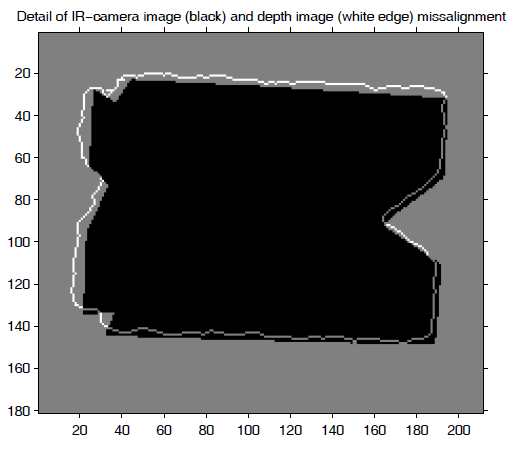
\includegraphics[width=0.3\linewidth]{figs/deslocamentokinectA.png}}
%	\subfloat[Com o alinhamento]{\label{fig:deslocamentokinectB}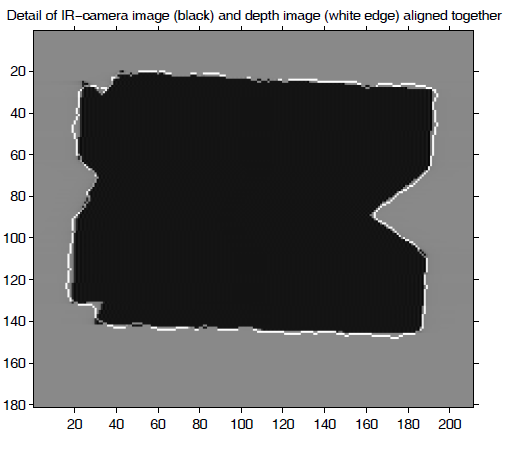
\includegraphics[width=0.3\linewidth]{figs/deslocamentokinectB.png}}
%	\caption{%
%	Representação visual do acerto do deslocamento. A parte em preto é a imagem IR e o contorno em branco é a imagem de profundidade do alvo.
%	}\label{fig:deslocKinect}
%\end{figure}

O Kinect é tão utilizado para fins pessoais (e empresariais), que existem alguns softwares para utilizá-lo como uma ferramenta de reconstrução 3D e a maioria deles são bem acessíveis (incluindo um pacote de ferramentas que a própria Microsoft disponibilizou, para o funcionamento do Kinect no Windows). Uma delas é o \emph{Skanect} que tem a versão gratuita onde é possível fazer escaneamentos básicos e a versão paga, que possibilita uma configuração maior, como por exemplo, a delimitação do objeto que será reconstruído, exportar o arquivo em diferentes formatos (\emph{.PLY}; \emph{.OBJ}: formato para exportação para programas que melhoram o modelo gerado (blender ou sculptris, por exemplo). E escolher o numero de faces a ser exportado; \emph{STL}: próprio para a impressora 3D (software \emph{Cura}); \emph{VRML}: salva também as cores do modelo.)

Entretanto, uma desvantagem que diminui a aplicabilidade do Kinect é que ele foi projetado para funcionar bem em espaços fechados, com detecção de formas humanas e movimentações. Ou seja, numa aplicação \emph{in situ} já não funcionaria muito bem, pois além de não conseguir projetar os detalhes em alta definição de uma escultura, ele necessita de uma fonte de energia externa, o que dificulta a acessibilidade, e, como  é gerada uma reconstrução em tempo real (não tem uma forma de salvar em \emph{cache} ou internamente), ele precisa estar ligado a um computador para fazer o escaneamento.
